\section{Independence of Causal Influence}\label{sec:independenceOfCausalInfluence}
Tree CPS (\S-~\nameref{sec:treeCPD}) are good for adding context with many parents. But when the number of the parents is quite large and most of the parents contribute (see Figure~\ref{fig:100_10}), then the Tree CPD is not a good representation.  For example, \emph{Cough} can be caused by an array of diseases.  We utilize a noisy OR CPD for this purpose.

\begin{marginfigure}
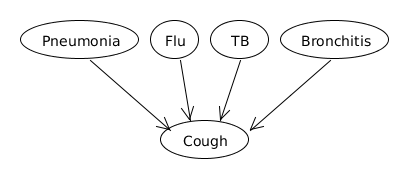
\includegraphics{images/100_10}
\caption{Multiple parents contributing towards a single variable.  This does not lead it self into a Tree CPD.}
\label{fig:100_10}
\end{marginfigure}

\subsection{Noisy OR CPD}
\begin{marginfigure}
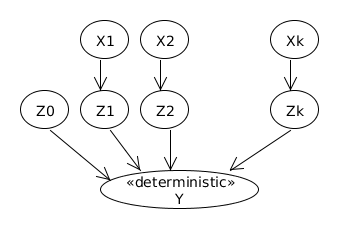
\includegraphics{images/100_11}
\caption{Noisy OR CPD}
\label{fig:100_11}
\end{marginfigure}

For each parent variable  \m{X}, we introduce an intermediate variable \m{Z} (filter). \m{Z} represents the event of a parent \m{X} being \emph{true}, causing \m{Y} to be true by itself.  Ultimately \m{Y} is true if any \m{Z} succeeded in making it true.  Therefore, \m{Y} is a deterministic \m{OR} based of its parents \m{Z}.
\marginnote{\emph{Penetrance} defines how good is \m{X_i} in turning \m{Z_i}, where as \emph{Leak} defines \m{Y} turning on by itself.}
\[ P(Z_0 =1) = \lambda_0  \quad Leak\]

\[
  P(Z_i =1 |X_i	) = \left\{
  \begin{array}{l l}
    0  & \quad X_i=0\\
    \lambda_i & \quad X_i=1 \quad Penetrance\\
  \end{array} \right.
\]

Now consider, what is the probability that \m{Y=0} given all the parents \m{X}:
\[P(Y=0|X_1,X_2 \ldots, X_k) = (1-\lambda_0	) \prod\limits_{i:X_i=1} (1-\lambda_i) \] where, $\prod\limits_{i:X_i=1} (1-\lambda_i)$ represents the parents that are on.

For the probability that \m{Y=1}, we have
\[  P(Y=1|X_1,X_2 \ldots, X_k) =   1- P(Y=0|X_1,X_2 \ldots, X_k)  \]

\newthought{Generalization of the noisy OR CPD: } Figure~\ref{fig:100_12} represents the generalization of the noisy OR CPD.  The variable \m{Z} is a deterministic variable that can represent different functions such as and \emph{AND} operation, \emph{MAX} operation etc.

\begin{marginfigure}
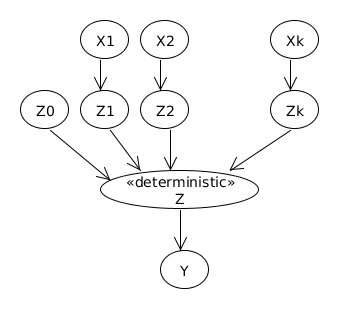
\includegraphics{images/100_12}
\caption{Generalization of the noisy OR CPD}
\label{fig:100_12}
\end{marginfigure}

\subsection{Sigmoid CPD} 

Given \m{Z = w_0 + \sum\limits_{i=1}^k w_i X_i}, where \m{Z_i=w_i X_i}., a sigmoid CPD is
\[P(y^1 | X_1, X_2, \ldots, X_k) = sigmoid(Z) \]
Where \m{sigmoid(z) = \frac{e^z}{1+e^z}}, \m{z} is a continuous variable.  The result of the \m{sigmoid} function is to reduce the value of \m{z} to \m{[0,1]}.

\section{Continuous Variables}
\begin{marginfigure}
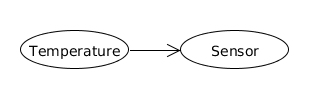
\includegraphics{images/100_20}
\caption{Example of continuous variables}
\label{fig:100_20}
\end{marginfigure}

Imagine that the temperature is a \emph{continuous variable} and the sensor provides an approximation of the temperature.  That is \emph{sensor} \m{S} is a normal distribution defined using \emph{linear Gaussian} as: \[ S \sim \mathcal{N} (T; \sigma^2_s )\]


\begin{marginfigure}
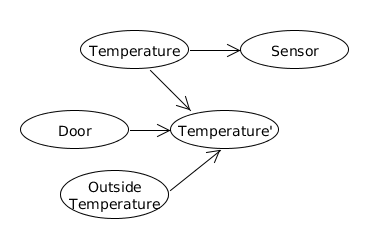
\includegraphics{images/100_21}
\caption{Example of continuous variables with condition}
\label{fig:100_21}
\end{marginfigure}
No imagine that the temperature soon \m{Temperature'} depends on current temperature, outside temperature and the conditionally on the door being opened or closed (as shown in Figure~\ref{fig:100_21}).  We have the following \emph{conditional linear Gaussian} distributions:

\[ T' \sim \mathcal{N} (\alpha_0T + (1-\alpha_0)O; \sigma^2_{0T} ) \quad \text{when } D^0\]
\[ T' \sim \mathcal{N} (\alpha_1T + (1-\alpha_1)O; \sigma^2_{1T} ) \quad \text{when } D^1\]


\subsection{Linear Gaussian}
\begin{marginfigure}
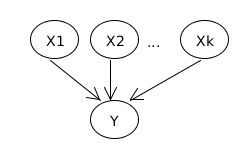
\includegraphics{images/100_22}
\caption{Model for linear Gaussian.}
\label{fig:100_22}
\end{marginfigure}
For the given graph in Figure~\ref{fig:100_22}, we have a variable \m{Y} with parents \m{X}, then we have a \emph{linear Gaussian} defined as follows:
\[ Y \sim \mathcal{N} (w_0 +  \sum w_i X_i; \sigma^2 )\]
where,  the mean of the Gaussian distribution (\m{w_0 +  \sum w_i X_i}) is a linear function (of the parents \m{X_i}, and the variance $\sigma^2$ does not depend on the parents.

\subsection{Conditional Linear Gaussian}
\begin{marginfigure}
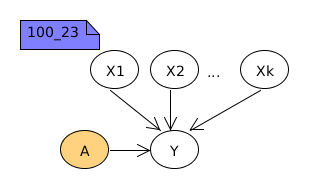
\includegraphics{images/100_23}
\caption{Model for conditional linear Gaussian.  Variable \m{A} is a discrete parent.  There can be more than one discrete parents.}
\label{fig:100_23}
\end{marginfigure}
We can now define a \emph{conditional linear Gaussian} (see Figure~\ref{fig:100_23}) with a discrete parent variable \m{A} as follows:
\[ Y \sim \mathcal{N} (w_{a0} +  \sum w_i X_i; \sigma^2_a )\]
Note that the variance $\sigma^2_a$ depends on the discrete parent \m{A} but not \m{X}.




